\paragraph{Neural Episodic Control} Neural Episodic Control \cite{pritzel2017neural}
Deep reinforcement learning methods attain super-human performance in a wide range of environments. \uline{Such methods are grossly inefficient,  often taking orders of magnitudes more data than human to achieve reasonable performance.} \textcolor{red}{\uline{Neural Episodic Control : a deep reinforcement learning agent that is able to rapidly assimilate new experiences and act upon them. Our agent uses a semi-tabular representation of the value function: a buffer of past experience containing slowly changing state representations and rapidly updated estimates of the value function. }}
\paragraph{} The agent of NEC consists of three components: a convolutional neural network that processes pixel images $s$, a set of memory modules (one per action), and a final network that converts read-outs from the actions memories into $Q(s, a)$ values.
\paragraph{Differentiable Neural Dictionary (DND)} For each action $a \in \mathcal{A}$, NEC has a simple memory module $M_{a} = (K_{a}, V_{a})$, where $K_{a}$ and $V_{a}$ are dynamically sized arrays of vectors, each containing the same number of vectors. The memory module acts as an arbitrary association from keys to corresponding values, much like the dictionary data type found in programs. Thus we refer to this kind of memory module as a \textit{differentiable neural dictionary} (DND). There are two operations possible on a DND: \textit{lookup} and \textit{write}, Performing a lookup on a DND maps a key $h$ to an output value $o$:
\begin{equation} \label{output_o}
o = \sum_{i}w_{i}v_{i}
\end{equation}
where $v_{i}$ is the $i$th element of the array $V_{a}$ and 
\begin{equation} \label{weight_w}
w_{i} = k(h, h_{i})/\sum_{j}k(h, h_{j})
\end{equation}
where $h_{i}$ is the $i$th element of the array $K_{a}$ and $k(x, y)$ is a kernel between vectors $x$ and $y$, e.g., Gaussian or inverse kernels, such as:
\begin{equation}
k(h, h_{i}) = \frac{1}{||h - h_{i}||_{2}^{2} + \delta}
\end{equation}
Thus the output of a lookup in a DND is a weighted sum of the values in the memory, whose weights are given by normalised kernels between the lookup key and the corresponding key in memory. To make queries into very large memories scalable we shall make two approximations in practice: firstly, we shall limit (\ref{output_o}) to the top $p$-nearest neighbours. Secondly, we use an approximate nearest neighbours algorithm to perform the lookups, based up kd-trees.
\paragraph{} keys and values are written to the memory by appending them onto the end of the arrays $K_{a}$ and $V_{a}$ respectively. if a key already exists in the memory, then its corresponding value is updated, rather than being duplicated.
\paragraph{Agent Architecture}
Figure (\ref{nec_agent_architecture_figure}) shows a DND as part of the NEC agent for asingle action, whilst Algorithm (\ref{nec_algorithm}) describes the general outline of the NEC algorithm. 
\paragraph{} The pixel state $s$ is processed by a convolutional neural network to produce a key $h$. The key $h$ is then used to lookup a value from the DND, yielding weights $w_i$ in the process for each element of the memory arrays. Finally, the output is a weighted sum of the values in the DND. The values in the DND, in the case of an NEC agent, are the $Q$ values corresponding to the state that originally resulted in the corresponding key-value pair to be written to hte memory. Thus this architecture produces an estimate of $Q(s, a)$ for a single given action $a$/ The architecture is replicated once for each action $a$ the agent can take, with the convolutional part of the network shared among each separate DND $M_a$. The NEX agent acts by taking the action with the highest $Q$-value estimate at each time step. In practice, we use $\epsilon$-greedy policy during training with a low $\epsilon$.
\begin{figure}
\centering
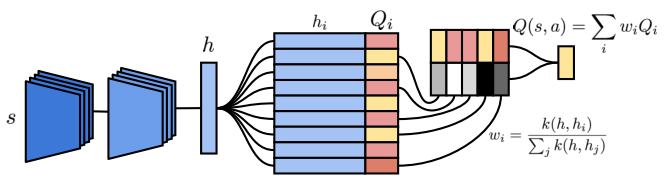
\includegraphics[width=10cm]{pic/nec_agent_architecture.PNG}
\caption{Architecture of episodic memory module for a single action $a$. Pixels representing the current state enter through a convolutional neural network on the bottom left and an estimate of $Q(s, a)$ exists top right. Gradients flow through the entire architecture.} 
\label{nec_agent_architecture_figure}
\end{figure}
\begin{algorithm}
\caption{Neural Episodic Control} \label{nec_algorithm}
\begin{algorithmic}[h]
	\State $\mathcal{D}$: replay memory
	\State $M_{a}$: a DND for each action $a$.
	\State $N$: horizon for $N$-step $Q$ estimate.
	\For {each episode}
		\For {$t = 1, 2, ..., T$}
			\State Receive observation $s_t$ from environment with embedding $h$.
			\State Estimate $Q(s_t, a)$ for each action $a$ via (\ref{output_o}) from $M_{a}$
			\State $a_{t} \leftarrow \epsilon-$greedy policy based on $Q(s_t, a)$
			\State Take action $a_{t}$, receive reward $r_{t+1}$.
			\State Append $(h, Q^{(N)}(s_t, a_t))$ to $M_{a_t}$.
			\State Append $(s_t, a_t, Q^{(N)}(s_t, a_t))$ to $\mathcal{D}$.
		\EndFor
	\EndFor
\end{algorithmic}
\end{algorithm}

\paragraph{}The N-step Q-value estimate is 
\begin{equation} \label{q_n_s_t_a_eq}
Q^{(N)}(s_t, a) = \sum_{j=0}^{N-1}\gamma^{j}r_{t+j} + \gamma^{N}\max_{a^{'}}Q(s_{t+N}, a^{'}).
\end{equation}
The bootstrap term of (\ref{q_n_s_t_a_eq}), $\max_{a^{'}}Q(s_{t+N}, a^{'})$ is found by querying all memories $M_{a}$ for each action $a$ and taking the highest estimated $Q$-value returned. Note that the earliest such values can be added to memory is $N$ steps after a particular $(s, a)$ pair occurs.
\paragraph{}When a state-action value is already present in a DND (i.e the exact same key $h$ is already in $K_a$), the corresponding value present in $V_a, Q_i$, is updated in the same way as the classic tabular Q-learning algorithm:
\begin{equation}\label{update_q_i_eq}
Q_{i}\leftarrow Q_{i} + \alpha(Q^{(N)}(s, a)- Q_{i})
\end{equation}
where $\alpha$ is the learning rate of the $Q$ update.